% Options for packages loaded elsewhere
\PassOptionsToPackage{unicode}{hyperref}
\PassOptionsToPackage{hyphens}{url}
%
\documentclass[
  english,
  doc]{apa6}
\usepackage{amsmath,amssymb}
\usepackage{lmodern}
\usepackage{ifxetex,ifluatex}
\ifnum 0\ifxetex 1\fi\ifluatex 1\fi=0 % if pdftex
  \usepackage[T1]{fontenc}
  \usepackage[utf8]{inputenc}
  \usepackage{textcomp} % provide euro and other symbols
\else % if luatex or xetex
  \usepackage{unicode-math}
  \defaultfontfeatures{Scale=MatchLowercase}
  \defaultfontfeatures[\rmfamily]{Ligatures=TeX,Scale=1}
\fi
% Use upquote if available, for straight quotes in verbatim environments
\IfFileExists{upquote.sty}{\usepackage{upquote}}{}
\IfFileExists{microtype.sty}{% use microtype if available
  \usepackage[]{microtype}
  \UseMicrotypeSet[protrusion]{basicmath} % disable protrusion for tt fonts
}{}
\makeatletter
\@ifundefined{KOMAClassName}{% if non-KOMA class
  \IfFileExists{parskip.sty}{%
    \usepackage{parskip}
  }{% else
    \setlength{\parindent}{0pt}
    \setlength{\parskip}{6pt plus 2pt minus 1pt}}
}{% if KOMA class
  \KOMAoptions{parskip=half}}
\makeatother
\usepackage{xcolor}
\IfFileExists{xurl.sty}{\usepackage{xurl}}{} % add URL line breaks if available
\IfFileExists{bookmark.sty}{\usepackage{bookmark}}{\usepackage{hyperref}}
\hypersetup{
  pdftitle={Brief methods note: Investigators must exercise caution prior to dichotomizing continuous variables for use as binary outcomes in logistic regression},
  pdfauthor={James Uanhoro1},
  pdflang={en-EN},
  pdfkeywords={logistic regression, dichotomization, heteroskedasticity},
  hidelinks,
  pdfcreator={LaTeX via pandoc}}
\urlstyle{same} % disable monospaced font for URLs
\usepackage{graphicx}
\makeatletter
\def\maxwidth{\ifdim\Gin@nat@width>\linewidth\linewidth\else\Gin@nat@width\fi}
\def\maxheight{\ifdim\Gin@nat@height>\textheight\textheight\else\Gin@nat@height\fi}
\makeatother
% Scale images if necessary, so that they will not overflow the page
% margins by default, and it is still possible to overwrite the defaults
% using explicit options in \includegraphics[width, height, ...]{}
\setkeys{Gin}{width=\maxwidth,height=\maxheight,keepaspectratio}
% Set default figure placement to htbp
\makeatletter
\def\fps@figure{htbp}
\makeatother
\setlength{\emergencystretch}{3em} % prevent overfull lines
\providecommand{\tightlist}{%
  \setlength{\itemsep}{0pt}\setlength{\parskip}{0pt}}
\setcounter{secnumdepth}{-\maxdimen} % remove section numbering
% Make \paragraph and \subparagraph free-standing
\ifx\paragraph\undefined\else
  \let\oldparagraph\paragraph
  \renewcommand{\paragraph}[1]{\oldparagraph{#1}\mbox{}}
\fi
\ifx\subparagraph\undefined\else
  \let\oldsubparagraph\subparagraph
  \renewcommand{\subparagraph}[1]{\oldsubparagraph{#1}\mbox{}}
\fi
% Manuscript styling
\usepackage{upgreek}
\captionsetup{font=singlespacing,justification=justified}

% Table formatting
\usepackage{longtable}
\usepackage{lscape}
% \usepackage[counterclockwise]{rotating}   % Landscape page setup for large tables
\usepackage{multirow}		% Table styling
\usepackage{tabularx}		% Control Column width
\usepackage[flushleft]{threeparttable}	% Allows for three part tables with a specified notes section
\usepackage{threeparttablex}            % Lets threeparttable work with longtable

% Create new environments so endfloat can handle them
% \newenvironment{ltable}
%   {\begin{landscape}\centering\begin{threeparttable}}
%   {\end{threeparttable}\end{landscape}}
\newenvironment{lltable}{\begin{landscape}\centering\begin{ThreePartTable}}{\end{ThreePartTable}\end{landscape}}

% Enables adjusting longtable caption width to table width
% Solution found at http://golatex.de/longtable-mit-caption-so-breit-wie-die-tabelle-t15767.html
\makeatletter
\newcommand\LastLTentrywidth{1em}
\newlength\longtablewidth
\setlength{\longtablewidth}{1in}
\newcommand{\getlongtablewidth}{\begingroup \ifcsname LT@\roman{LT@tables}\endcsname \global\longtablewidth=0pt \renewcommand{\LT@entry}[2]{\global\advance\longtablewidth by ##2\relax\gdef\LastLTentrywidth{##2}}\@nameuse{LT@\roman{LT@tables}} \fi \endgroup}

% \setlength{\parindent}{0.5in}
% \setlength{\parskip}{0pt plus 0pt minus 0pt}

% \usepackage{etoolbox}
\makeatletter
\patchcmd{\HyOrg@maketitle}
  {\section{\normalfont\normalsize\abstractname}}
  {\section*{\normalfont\normalsize\abstractname}}
  {}{\typeout{Failed to patch abstract.}}
\patchcmd{\HyOrg@maketitle}
  {\section{\protect\normalfont{\@title}}}
  {\section*{\protect\normalfont{\@title}}}
  {}{\typeout{Failed to patch title.}}
\makeatother
\shorttitle{Dichotomizing continuous outcome variables}
\keywords{logistic regression, dichotomization, heteroskedasticity}
\usepackage{lineno}

\linenumbers
\usepackage{csquotes}
\ifxetex
  % Load polyglossia as late as possible: uses bidi with RTL langages (e.g. Hebrew, Arabic)
  \usepackage{polyglossia}
  \setmainlanguage[]{english}
\else
  \usepackage[main=english]{babel}
% get rid of language-specific shorthands (see #6817):
\let\LanguageShortHands\languageshorthands
\def\languageshorthands#1{}
\fi
\ifluatex
  \usepackage{selnolig}  % disable illegal ligatures
\fi
\newlength{\cslhangindent}
\setlength{\cslhangindent}{1.5em}
\newlength{\csllabelwidth}
\setlength{\csllabelwidth}{3em}
\newenvironment{CSLReferences}[2] % #1 hanging-ident, #2 entry spacing
 {% don't indent paragraphs
  \setlength{\parindent}{0pt}
  % turn on hanging indent if param 1 is 1
  \ifodd #1 \everypar{\setlength{\hangindent}{\cslhangindent}}\ignorespaces\fi
  % set entry spacing
  \ifnum #2 > 0
  \setlength{\parskip}{#2\baselineskip}
  \fi
 }%
 {}
\usepackage{calc}
\newcommand{\CSLBlock}[1]{#1\hfill\break}
\newcommand{\CSLLeftMargin}[1]{\parbox[t]{\csllabelwidth}{#1}}
\newcommand{\CSLRightInline}[1]{\parbox[t]{\linewidth - \csllabelwidth}{#1}\break}
\newcommand{\CSLIndent}[1]{\hspace{\cslhangindent}#1}

\title{Brief methods note: Investigators must exercise caution prior to dichotomizing continuous variables for use as binary outcomes in logistic regression}
\author{James Uanhoro\textsuperscript{1}}
\date{}


\authornote{

James Uanhoro is a PhD student in the Quantitative Research, Evaluation and Measurement program within the Department of Educational Studies

Correspondence concerning this article should be addressed to James Uanhoro, 210 Ramseyer Hall, 29 W Woodruff Ave, Columbus, OH 43210. E-mail: \href{mailto:uanhoro.1@osu.edu}{\nolinkurl{uanhoro.1@osu.edu}}

}

\affiliation{\vspace{0.5cm}\textsuperscript{1} The Ohio State University}

\abstract{
A common practice in empirical data analysis is to dichotomize continuous outcomes for substantive or interpretational purposes. A particular cut-point on the outcome variable may be practically relevant, such that researchers dichotomize the continuous outcome at the cut-point to create a binary outcome, then proceed to model this binary outcome using logistic regression. However, homoskedasticity of the error term in the linear regression model for the continuous outcome is an often overlooked assumption for this application of logistic regression to be valid. If this condition is not met, the logistic regression model for the binary outcome will be misspecified, and the coefficients and predicted probabilities will be incorrect. Correctly estimating the relationship can be difficult computationally. Hence, I recommend that researchers directly model the continuous outcome even when there are substantive justifications for modeling the dichotomized outcome.
}



\begin{document}
\maketitle

\hypertarget{introduction}{%
\section{Introduction}\label{introduction}}

It is a relatively common practice for education researchers to dichotomize continuous variables into binary variables, then analyze the binary variables using logistic regression. The most common reason for doing this is substantive. For example, the original response variable may be student scores on a test with range of 0 to 100. On this test, students with scores equal to or above 70 pass, while others fail. In such situations, researchers interested in understanding the dynamics of student success on the test may dichotomize the original test scores into 1 (pass) or 0 (fail) and model the probability that a student passed (or failed) using logistic regression.

In this paper, I argue that there are reasons to distrust the findings from such a procedure. In the next section, I review two formulations for the logistic regression model. By doing this, it becomes evident why this procedure can be problematic. The source of this problem is heteroskedasticity in the linear regression model for the original continuous variable. I conclude with a simple demonstraton using simulated data.

\hypertarget{formulation-of-the-logistic-regression-model}{%
\section{Formulation of the logistic regression model}\label{formulation-of-the-logistic-regression-model}}

The standard logistic regression model is a generalized linear model (Fox, 2015; McCullagh \& Nelder, 1989) for the probabilities responsible for an observed Bernoulli response variable:

\begin{equation} \label{eq:1}
\ln\Bigg[\frac{p}{1-p}\Bigg]=\alpha + X\beta
\end{equation}

where \(p\) are the probabilities of success underlying the observed Bernoulli variable for each case, \(\alpha\) is the intercept, \(X\) is an \(n\) by \(k\) matrix for \(n\) cases and \(k\) predictors (excluding the intercept), and \(\beta\) are \(k\) regression weights for each predictor. The logit transformation applied to the probabilities (left hand side of equation \eqref{eq:1}) equates the probabilities to the predictors, \(X\), multiplied by their weights, \(\beta\), plus the intercept, \(\alpha\).

We can rewrite equation \eqref{eq:1} by solving for \(p\):

\begin{equation} \label{eq:2}
p=\frac{e^{(\alpha+X\beta)}}{1+e^{(\alpha+X\beta)}}
\end{equation}

Equation \eqref{eq:2} is also known as the inverse logit transformation applied to \(\alpha+X\beta\), transforming it from a value that has a possible range of \(-\infty\) to \(\infty\) to a probability guaranteed to lie between 0 and 1. At this point, I motivate the logistic regression model using a latent variable formulation (Amemiya, 1981):

\begin{equation} \label{eq:3}
p=P(\alpha+X\beta+\epsilon>t)
\end{equation}

This formulation of the model is the one we rely on when we dichotomize a continuous variable for use as the outcome in a logistic regression model. The probabilities underlying the new binary outcome are the probabilities that a continuous variable with a systematic componenent, \(\alpha + X\beta\), and random error, \(\epsilon\), exceeds a threshold, \(t\). For logistic regression, we make the additional assumption that \(\epsilon\) is a standard logistic variable \((\epsilon\sim\mathcal{L}(0, 1))\); this means that \(\epsilon\) has mean 0 and variance of \(\pi^2/3\).

As one will observe from equation \eqref{eq:3}, changing the value of \(t\) simply changes the value of \(\alpha\). If the threshold increases by 3, then the intercept increases by 3. So for the model to be identified, we will assume the threshold is 0, \(t=0\). Given this information, we continue to solve for \(p\) in equation \eqref{eq:3}:

\begin{align}
\begin{split} \label{eq:4}
p
{}&=P(\alpha+X\beta+\epsilon>0)=P(\epsilon>-\alpha-X\beta) \\
{}&=P(\epsilon<\alpha+X\beta)\quad\text{since }\mathcal{L}(0, 1) \text{ is symmetric about 0}
\end{split}
\end{align}

The final line of equation \eqref{eq:4} is simply the cumulative distribution function of \(\mathcal{L}(0, 1)\) evaluated at \(\alpha + X\beta\), hence:

\begin{equation} \label{eq:5}
p=\frac{e^{(\alpha+X\beta)}}{1+e^{(\alpha+X\beta)}}
\end{equation}

This result in equation \eqref{eq:5} shows that the latent variable formulation for the logistic regression model is equivalent to the generalized linear model formulation for logistic regression in equation \eqref{eq:2}. It also reveals one major assumption for the standard logistic regression model to be valid: the random error must be homoskedastic i.e.~\(\epsilon\sim\mathcal{L}(0, 1)\). If this assumption is violated, then equation \eqref{eq:5} is wrong. Assuming \(\epsilon\sim\mathcal{L}(0, \sigma)\) instead where \(\sigma\) has a different value for each case, the correct equation is:

\begin{equation} \label{eq:6}
p=\frac{e^{\big(\frac{\alpha+X\beta}{\sigma}\big)}}{1+e^{\big(\frac{\alpha+X\beta}{\sigma}\big)}}
\end{equation}

Hence if the random error is heteroskedastic, the standard logistic regression model as implemented in statistical software packages will be inadequate if the model is applied to the dichotomized outcome.

\hypertarget{how-problematic-can-this-form-of-heteroskedasticity-be}{%
\section{How problematic can this form of heteroskedasticity be?}\label{how-problematic-can-this-form-of-heteroskedasticity-be}}

To illustrate the problem, I present a simple example. Assume the following regression equation for a continuous variable, \(z_i\): \(z_i = 0.75 \times x_i + \epsilon_i\), where \(i=1, 2, \dots, 5000\), \(x_i\sim\mathrm{Bern}(0.5)\) and \(\epsilon_i\sim\mathcal{L}(0, \gamma_0 + \gamma_1x_i)\), so the error variance depends on \(x_i\). We can consider \(x_i\) random assignment to treatment \((x_i=1)\) and control \((x_i=0)\) groups, and \(z_i\) to be exam performance. I dichotomize \(z_i\) at 0 to create a new binary response, \(y_i\), such that \(y_i = 1\) when \(z_i > 0\) and \(y_i = 0\) when \(z_i \leq 0\). So \(z_i\) is exam performance underlying the binary outcome, \(y_i\) which we will consider to an indicator of passing the exam. I set \(\{\gamma_0, \gamma_1\} = \{1, 0\}\) to create a dataset with homoskedastic errors; then set \(\{\gamma_0, \gamma_1\} = \{\sqrt{1.5}, \frac{(\sqrt{3}-1)}{\sqrt{2}}\}\) to create another dataset with heteroskedastic errors.

As is visible from Figure \ref{fig:fig1}, the average relationship between \(x_i\) and each \(z_i\) is not that different under homoskedasticity and heteroskedasticity, but the heteroskedastic \(z_i\) visibly displays lesser error variance for the treatment group. The treatment not only improved performance on average, it shrunk the variability of the treatment group.

\begin{figure}
\centering
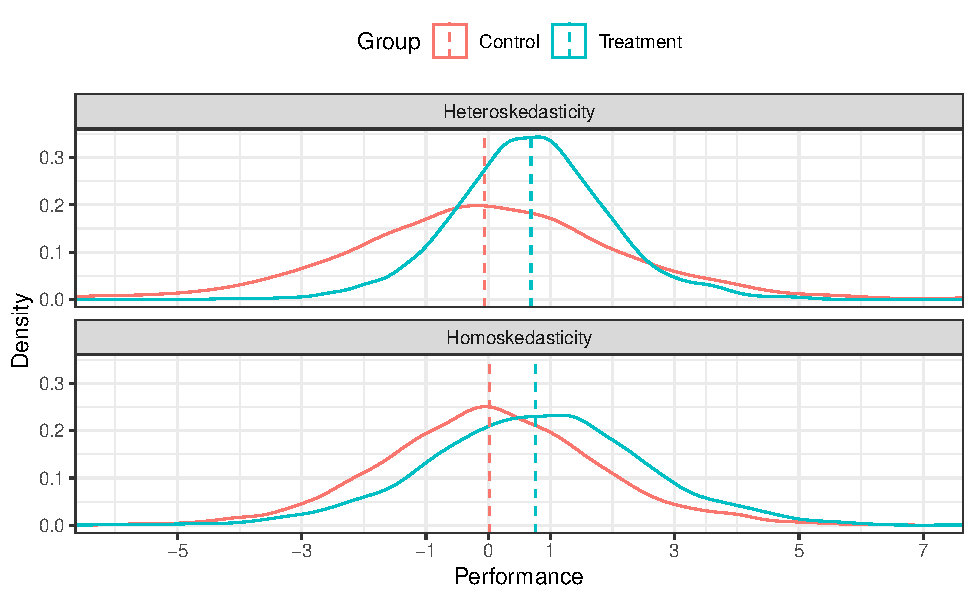
\includegraphics{dicho_het_log_files/figure-latex/fig1-1.pdf}
\caption{\label{fig:fig1}Relationship between group assignment and continuous outcome under heteroskedasticity (top panel) and homoskedasticity (bottom panel). The vertical dashed lines are group means. Under heteroskedasticity, the variance of z is smaller for the treatment group.}
\end{figure}

Next, I regressed the continuous variable, \(z_i\), on \(x_i\) using linear regression. Regardless of the error variance structure, the linear regression model had a decent recovery of the coefficient for \(x_i\); both coefficients were within 5\% of 0.75 (see first two columns of Table 1). This is consistent with the literature on linear regression models fit with OLS: unbiased coefficient estimation does not dependent on assumptions like homoskedasticity or normality of errors (Gelman \& Hill, 2007, p. 46).

\begin{table}[!htbp] \centering 
  \caption{Regression of outcome variables on x} 
  \label{} 
\small 
\begin{tabular}{@{\extracolsep{5pt}}lcccc} 
\\[-1.8ex]\hline 
\hline \\[-1.8ex] 
 & \multicolumn{4}{c}{\textit{Dependent variable:}} \\ 
\cline{2-5} 
\\[-1.8ex] & Homoskedastic z & Heteroskedastic z & Homoskedastic y & Heteroskedastic y \\ 
\hline \\[-1.8ex] 
 x & 0.739$^{***}$ & 0.752$^{***}$ & 0.719$^{***}$ & 1.011$^{***}$ \\ 
  & (0.050) & (0.052) & (0.058) & (0.060) \\ 
  & & & & \\ 
 Constant & 0.025 & $-$0.062 & 0.013 & $-$0.044 \\ 
  & (0.036) & (0.037) & (0.040) & (0.040) \\ 
  & & & & \\ 
\hline \\[-1.8ex] 
Observations & 5,000 & 5,000 & 5,000 & 5,000 \\ 
\hline 
\hline \\[-1.8ex] 
\textit{Note:}  & \multicolumn{4}{l}{$^{*}$p$<$0.05; $^{**}$p$<$0.01; $^{***}$p$<$0.001} \\ 
 & \multicolumn{4}{l}{The models for z are linear regression models. The models for y are logistic} \\ 
 & \multicolumn{4}{l}{regression models.} \\ 
\end{tabular} 
\end{table}

I next regressed the binary variable, \(y_i\), on \(x_i\) using logistic regression. Under homoskedastic error variance, the coefficient of \(x_i\) was 0.719, within 5\% of 0.75. However, under heteroskedastic error variance, the coefficient of \(x_i\) was about 35\% higher \(\big((1.011-0.75)/0.75\times 100\%\big)\) than what I specified in the data generation process. In this situation, we have inflation of the coefficient. Depending on the form of heteroskedasticity, the result might be coefficient deflation. Consequently, this misspecification returns incorrect probabilities of success for both groups. Under homoskedasticity, the treatment and control groups had 67.2\% \((1+e^{0.013+0.719})^{-1}\) and 50.3\% \((1+e^{0.013})^{-1}\) chance of passing the exam on average. Under heteroskedasticity, the treatment and control groups had 73.3\% \((1+e^{-0.044+1.011})^{-1}\) and 48.9\% \((1+e^{-0.044})^{-1}\) chance of passing the exam on average.

This happens because the standard logistic regression model is misspecified under heteroskedasticity. And one cannot recover the true logistic regression coefficients using standard maximum likelihood estimation of the logistic regression model.

\hypertarget{discussion}{%
\section{Discussion}\label{discussion}}

If the functional form of heteroskedasticity is known, then it is possible to modify the likelihood function used in maximum likelihood estimation of the logistic regression model. The literature is more developed in the case of probit models, where there exists a class of models known as \emph{heteroskedastic probit models} (Alvarez \& Brehm, 1995). However, even if the researcher can identify the functional form for heteroskedasticity, there is no guarantee that estimating the model will result in a correct solution because a ratio of parameters exists in the log-likelihood function (Keele \& Park, 2006). And potential problems include multiple solutions with near equivalent fit to the data, near singular Hessian matrices, large standard errors and convergence failures.

Hence, I recommend that when researchers have access to the original continuous variable, they should model this variable regardless of questions of substantive interest. If education researchers are interested in studying relationships at thresholds that are very different from the mean of the outcome, quantile regression (Koenker \& Hallock, 2001) is one approach for exploring the relationship between the predictors and continuous outcome at different quantiles of the outcome. There are methods for converting linear regression coefficients to logits and odds ratios (Moser \& Coombs, 2004) but they also rely on the aforementioned homoskedasticity assumption.

Finally, the problem of heteroscedasticity described above can exist even when the outcome variable is truly binary, or the binary outcome is difficult to rationalize as the manifestation of a dichotomized continuous variable. I focus on the case where the investigator has access to the continuous variable here because the situation is readily salvageable: analyze the continuous outcome directly. In situations where the investigator does not have access to the underlying continuous variable, but heteroskedasticity may be a concern, more flexible regression approaches such as generalized additive models (Hastie, 2017) and kernel regularized least squares (with logistic loss, Hainmueller \& Hazlett, 2014) may yield results that are more likely to reflect the true relations in the data. An additional alternative is to adopt a Bayesian framework using weakly informative priors to improve identification of the parameters in the log-likelihood function for heteroskedastic models.

\hypertarget{references}{%
\section{References}\label{references}}

\begingroup
\setlength{\parindent}{-0.5in}
\setlength{\leftskip}{0.5in}

\hypertarget{refs}{}
\begin{CSLReferences}{1}{0}
\leavevmode\hypertarget{ref-alvarez1995american}{}%
Alvarez, R. M., \& Brehm, J. (1995). American ambivalence towards abortion policy: Development of a heteroskedastic probit model of competing values. \emph{American Journal of Political Science}, 1055--1082.

\leavevmode\hypertarget{ref-Amemiya1981}{}%
Amemiya, T. (1981). {Qualitative Response Models: A Survey}. \emph{Journal of Economic Literature}, \emph{19}(4), 1483--1536. \url{https://doi.org/10.2307/2724565}

\leavevmode\hypertarget{ref-fox2015applied}{}%
Fox, J. (2015). \emph{Applied regression analysis and generalized linear models}. Sage Publications.

\leavevmode\hypertarget{ref-Gelman2007}{}%
Gelman, Andrew., \& Hill, J. (2007). \emph{{Data analysis using regression and multilevel/hierarchical models}} (p. 625). Cambridge University Press.

\leavevmode\hypertarget{ref-Hainmueller2014}{}%
Hainmueller, J., \& Hazlett, C. (2014). {Kernel regularized least squares: Reducing misspecification bias with a flexible and interpretable machine learning approach}. \emph{Political Analysis}, \emph{22}(2), 143--168. \url{https://doi.org/10.1093/pan/mpt019}

\leavevmode\hypertarget{ref-hastie2017generalized}{}%
Hastie, T. J. (2017). Generalized additive models. In \emph{Statistical models in s} (pp. 249--307). Routledge.

\leavevmode\hypertarget{ref-Keele2006}{}%
Keele, L., \& Park, D. K. (2006). \emph{{Ambivalent about ambivalence: A re-examination of heteroskedastic probit models}}. {Unpublished manuscript}.

\leavevmode\hypertarget{ref-koenker2001quantile}{}%
Koenker, R., \& Hallock, K. F. (2001). Quantile regression. \emph{Journal of Economic Perspectives}, \emph{15}(4), 143--156.

\leavevmode\hypertarget{ref-mccullagh1989nelder}{}%
McCullagh, P., \& Nelder, J. A. (1989). \emph{Generalized linear models}. Chapman {\&} Hall/CRC.

\leavevmode\hypertarget{ref-Moser2004}{}%
Moser, B. K., \& Coombs, L. P. (2004). {Odds ratios for a continuous outcome variable without dichotomizing}. \emph{Statistics in Medicine}, \emph{23}(12), 1843--1860. \url{https://doi.org/10.1002/sim.1776}

\end{CSLReferences}

\endgroup


\end{document}
